\documentclass{standalone}
\usepackage{tikz}
\begin{document}

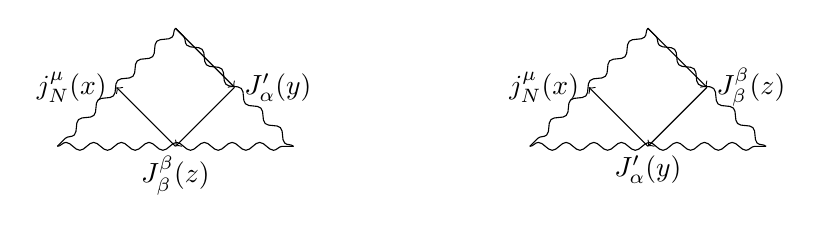
\begin{tikzpicture}
    % First diagram
    \begin{scope}[xshift=-3cm]
        % Left wavy line
        \draw[decorate, decoration={snake, amplitude=.5mm}] (0,0) -- (-1.5,-1.5) node[midway, left] {$j^\mu_N(x)$};
        % Right wavy line
        \draw[decorate, decoration={snake, amplitude=.5mm}] (1.5,-1.5) -- (0,0) node[midway, right] {$J'_\alpha(y)$};
        % Bottom wavy line
        \draw[decorate, decoration={snake, amplitude=.5mm}] (-1.5,-1.5) -- (1.5,-1.5) node[midway, below] {$J^\beta_\beta(z)$};
        % Triangle
        \draw[->] (0,0) -- (0.75,-0.75);
        \draw[->] (0.75,-0.75) -- (0,-1.5);
        \draw[->] (0,-1.5) -- (-0.75,-0.75);
    \end{scope}

    % Second diagram
    \begin{scope}[xshift=3cm]
        % Left wavy line
        \draw[decorate, decoration={snake, amplitude=.5mm}] (0,0) -- (-1.5,-1.5) node[midway, left] {$j^\mu_N(x)$};
        % Right wavy line
        \draw[decorate, decoration={snake, amplitude=.5mm}] (1.5,-1.5) -- (0,0) node[midway, right] {$J^\beta_\beta(z)$};
        % Bottom wavy line
        \draw[decorate, decoration={snake, amplitude=.5mm}] (-1.5,-1.5) -- (1.5,-1.5) node[midway, below] {$J'_\alpha(y)$};
        % Triangle
        \draw[->] (0,0) -- (0.75,-0.75);
        \draw[->] (0.75,-0.75) -- (0,-1.5);
        \draw[->] (0,-1.5) -- (-0.75,-0.75);
    \end{scope}
\end{tikzpicture}

\end{document}